\documentclass{standalone}
\usepackage{tikz}
\usetikzlibrary{patterns, positioning}
\usepackage[sfdefault]{ClearSans} %% option 'sfdefault' activates Clear Sans as the default text font
\usepackage[T1]{fontenc}

\begin{document}
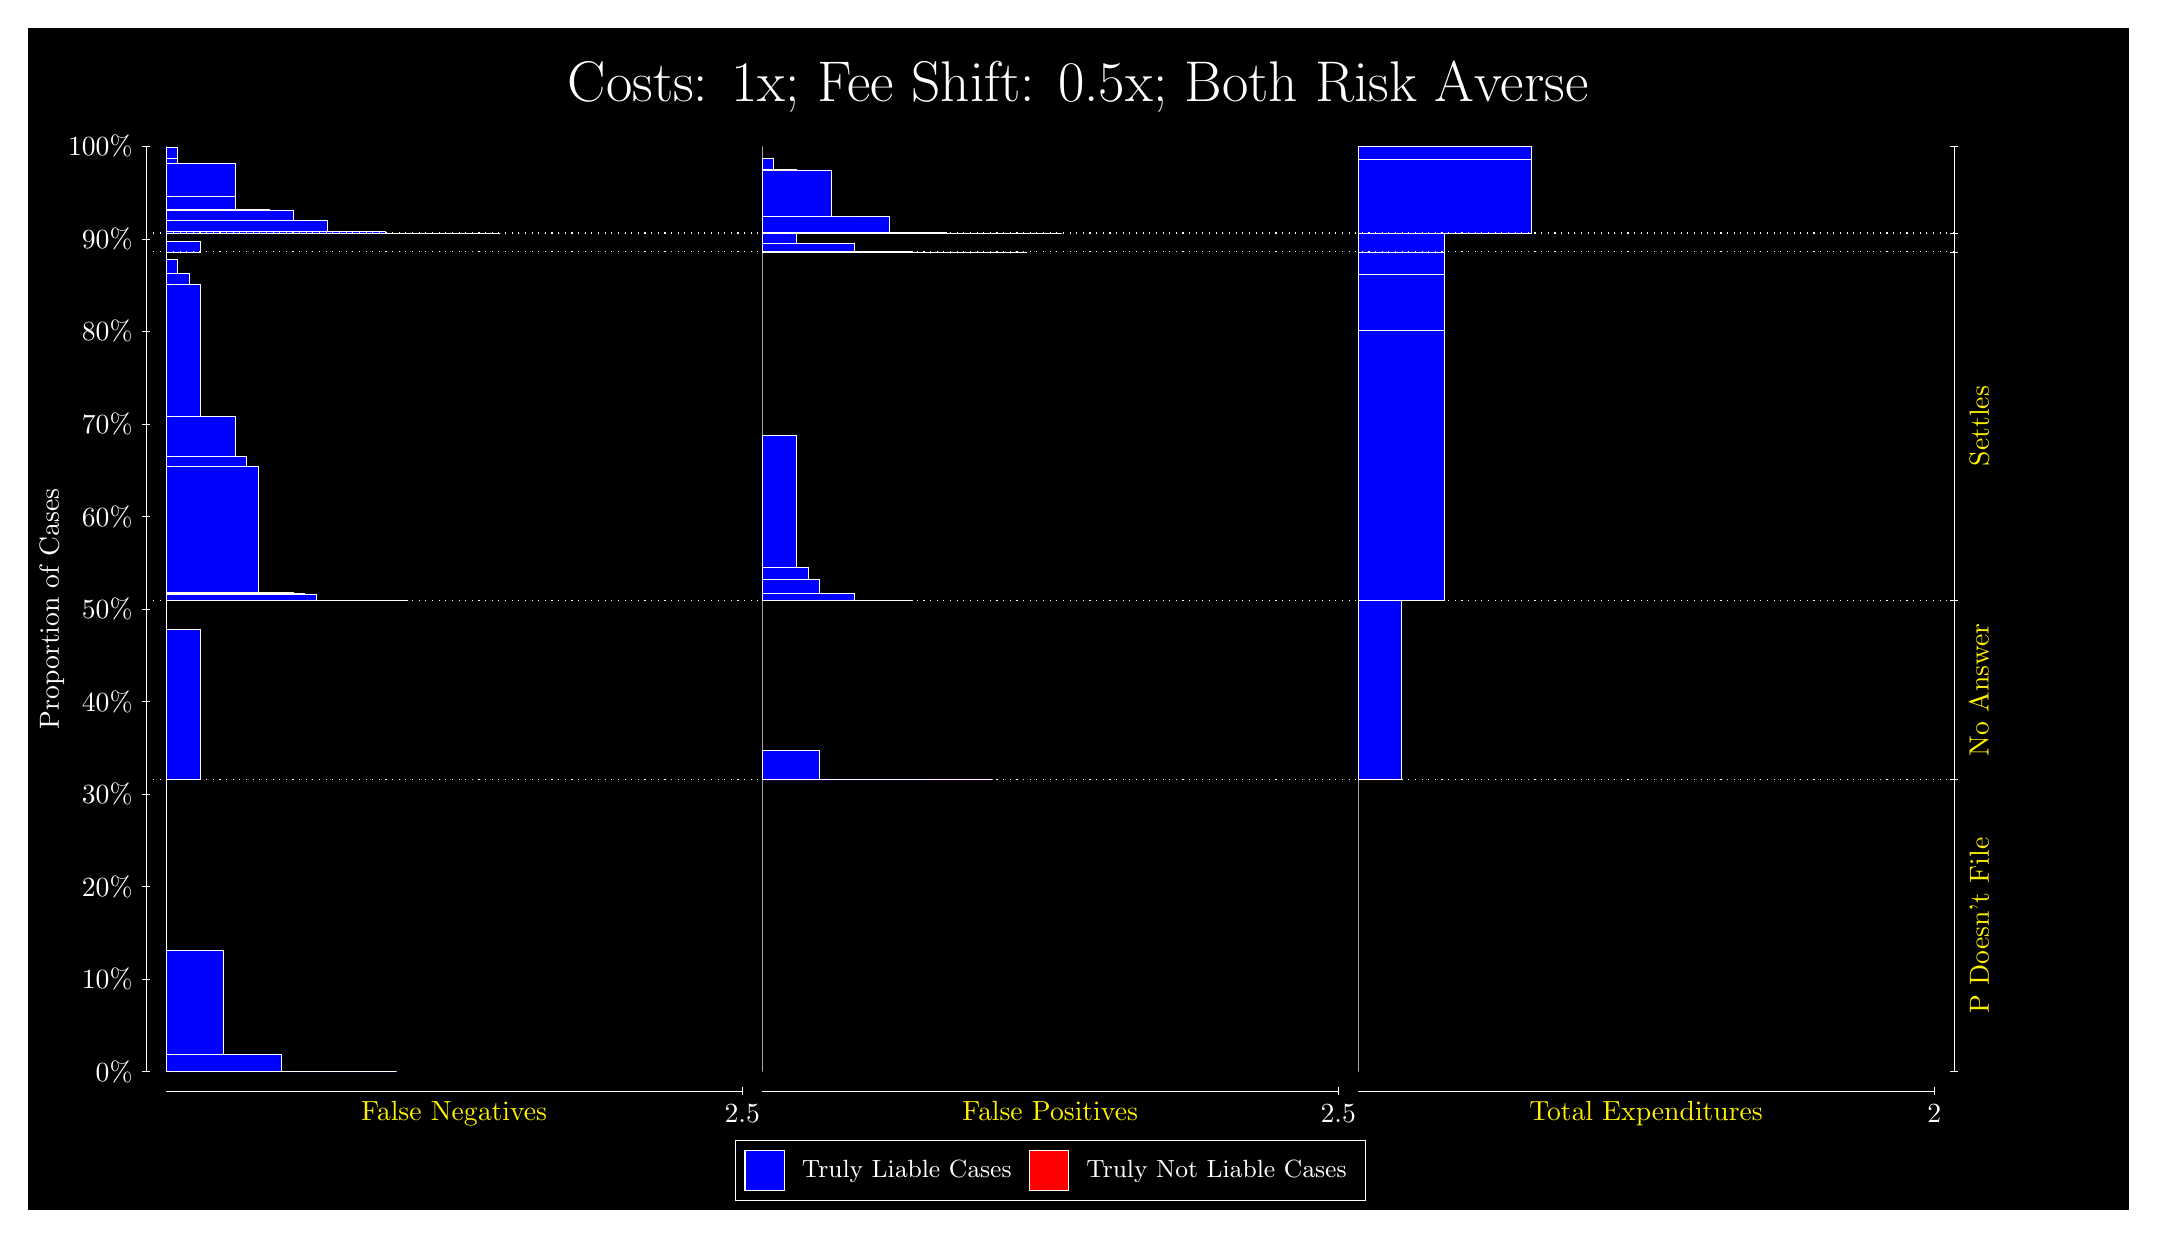
\begin{tikzpicture}
\draw[fill=black] (0,0) rectangle (26.667,15);
\draw[text=white] (0,13.5) rectangle (26.667,15) node[midway] {\huge Costs: 1x; Fee Shift: 0.5x; Both Risk Averse};
\draw[white, very thin] (1.5,1.75) -- (1.5,13.5);
\node[rotate=90, text=white, anchor=center] at (0.3, 7.625) {Proportion of Cases};
\draw[white, very thin] (1.45,1.75) -- (1.55,1.75);
\node[text=white, anchor=east] at (1.45, 1.75) {0\%};
\draw[white, very thin] (1.45,2.925) -- (1.55,2.925);
\node[text=white, anchor=east] at (1.45, 2.925) {10\%};
\draw[white, very thin] (1.45,4.1) -- (1.55,4.1);
\node[text=white, anchor=east] at (1.45, 4.1) {20\%};
\draw[white, very thin] (1.45,5.275) -- (1.55,5.275);
\node[text=white, anchor=east] at (1.45, 5.275) {30\%};
\draw[white, very thin] (1.45,6.45) -- (1.55,6.45);
\node[text=white, anchor=east] at (1.45, 6.45) {40\%};
\draw[white, very thin] (1.45,7.625) -- (1.55,7.625);
\node[text=white, anchor=east] at (1.45, 7.625) {50\%};
\draw[white, very thin] (1.45,8.8) -- (1.55,8.8);
\node[text=white, anchor=east] at (1.45, 8.8) {60\%};
\draw[white, very thin] (1.45,9.975) -- (1.55,9.975);
\node[text=white, anchor=east] at (1.45, 9.975) {70\%};
\draw[white, very thin] (1.45,11.15) -- (1.55,11.15);
\node[text=white, anchor=east] at (1.45, 11.15) {80\%};
\draw[white, very thin] (1.45,12.325) -- (1.55,12.325);
\node[text=white, anchor=east] at (1.45, 12.325) {90\%};
\draw[white, very thin] (1.45,13.5) -- (1.55,13.5);
\node[text=white, anchor=east] at (1.45, 13.5) {100\%};

\draw[white, very thin] (24.457,1.75) -- (24.457,13.5);
\draw[white, very thin] (24.407,1.75) -- (24.507,1.75);
\node[anchor=west] at (24.407, 1.75) {};
\draw[white, very thin] (24.407,5.4578) -- (24.507,5.4578);
\node[anchor=west] at (24.407, 5.4578) {};
\draw[white, very thin] (24.407,7.7374) -- (24.507,7.7374);
\node[anchor=west] at (24.407, 7.7374) {};
\draw[white, very thin] (24.407,12.16) -- (24.507,12.16);
\node[anchor=west] at (24.407, 12.16) {};
\draw[white, very thin] (24.407,12.399) -- (24.507,12.399);
\node[anchor=west] at (24.407, 12.399) {};
\draw[white, very thin] (24.407,13.5) -- (24.507,13.5);
\node[anchor=west] at (24.407, 13.5) {};

\draw[white, very thin, fill=blue] (1.75,1.75) rectangle (4.6775,1.75);
\draw[white, very thin, fill=blue] (1.75,1.75) rectangle (3.9457,1.7519);
\draw[white, very thin, fill=blue] (1.75,1.7519) rectangle (3.2138,1.9733);
\draw[white, very thin, fill=blue] (1.75,1.9733) rectangle (2.4819,3.2916);
\draw[white, very thin, fill=red] (1.75,3.2916) rectangle (1.75,3.2916);
\draw[white, very thin, fill=blue] (1.75,3.2916) rectangle (1.75,5.4578);
\draw[white, very thin, fill=blue] (1.75,5.4578) rectangle (2.1891,7.3646);
\draw[white, very thin, fill=red] (1.75,7.3646) rectangle (1.75,7.3646);
\draw[white, very thin, fill=blue] (1.75,7.3646) rectangle (1.75,7.7374);
\draw[white, very thin, fill=blue] (1.75,7.7374) rectangle (4.8239,7.7374);
\draw[white, very thin, fill=blue] (1.75,7.7374) rectangle (4.2384,7.7374);
\draw[white, very thin, fill=blue] (1.75,7.7374) rectangle (4.092,7.7374);
\draw[white, very thin, fill=blue] (1.75,7.7374) rectangle (3.6529,7.8167);
\draw[white, very thin, fill=blue] (1.75,7.8167) rectangle (3.5065,7.8178);
\draw[white, very thin, fill=blue] (1.75,7.8178) rectangle (3.3602,7.8394);
\draw[white, very thin, fill=blue] (1.75,7.8394) rectangle (2.921,9.4325);
\draw[white, very thin, fill=blue] (1.75,9.4325) rectangle (2.7746,9.5622);
\draw[white, very thin, fill=blue] (1.75,9.5622) rectangle (2.6283,10.07);
\draw[white, very thin, fill=blue] (1.75,10.07) rectangle (2.1891,11.743);
\draw[white, very thin, fill=blue] (1.75,11.743) rectangle (2.0428,11.894);
\draw[white, very thin, fill=blue] (1.75,11.894) rectangle (1.8964,12.07);
\draw[white, very thin, fill=red] (1.75,12.07) rectangle (1.75,12.07);
\draw[white, very thin, fill=blue] (1.75,12.07) rectangle (1.75,12.16);
\draw[white, very thin, fill=blue] (1.75,12.16) rectangle (2.1891,12.288);
\draw[white, very thin, fill=red] (1.75,12.288) rectangle (1.75,12.288);
\draw[white, very thin, fill=blue] (1.75,12.288) rectangle (1.75,12.399);
\draw[white, very thin, fill=blue] (1.75,12.399) rectangle (5.9949,12.399);
\draw[white, very thin, fill=blue] (1.75,12.399) rectangle (5.2631,12.4);
\draw[white, very thin, fill=blue] (1.75,12.4) rectangle (4.8239,12.4);
\draw[white, very thin, fill=blue] (1.75,12.4) rectangle (4.5312,12.42);
\draw[white, very thin, fill=blue] (1.75,12.42) rectangle (4.092,12.42);
\draw[white, very thin, fill=blue] (1.75,12.42) rectangle (3.7993,12.555);
\draw[white, very thin, fill=blue] (1.75,12.555) rectangle (3.3602,12.693);
\draw[white, very thin, fill=blue] (1.75,12.693) rectangle (3.0674,12.704);
\draw[white, very thin, fill=blue] (1.75,12.704) rectangle (2.6283,12.86);
\draw[white, very thin, fill=blue] (1.75,12.86) rectangle (2.6283,13.284);
\draw[white, very thin, fill=blue] (1.75,13.284) rectangle (2.3355,13.284);
\draw[white, very thin, fill=blue] (1.75,13.284) rectangle (1.8964,13.349);
\draw[white, very thin, fill=blue] (1.75,13.349) rectangle (1.8964,13.486);
\draw[white, very thin, fill=red] (1.75,13.486) rectangle (1.75,13.486);
\draw[white, very thin, fill=blue] (1.75,13.486) rectangle (1.75,13.5);
\draw[white, very thin, fill=red] (9.3189,1.75) rectangle (9.3189,1.75);
\draw[white, very thin, fill=blue] (9.3189,1.75) rectangle (9.3189,5.4578);
\draw[white, very thin, fill=red] (9.3189,5.4578) rectangle (12.246,5.4578);
\draw[white, very thin, fill=blue] (9.3189,5.4578) rectangle (12.246,5.4578);
\draw[white, very thin, fill=blue] (9.3189,5.4578) rectangle (11.515,5.4578);
\draw[white, very thin, fill=blue] (9.3189,5.4578) rectangle (10.783,5.4607);
\draw[white, very thin, fill=blue] (9.3189,5.4607) rectangle (10.051,5.8306);
\draw[white, very thin, fill=blue] (9.3189,5.8306) rectangle (9.3189,7.7374);
\draw[white, very thin, fill=red] (9.3189,7.7374) rectangle (11.222,7.7374);
\draw[white, very thin, fill=blue] (9.3189,7.7374) rectangle (11.222,7.7375);
\draw[white, very thin, fill=red] (9.3189,7.7375) rectangle (10.636,7.7375);
\draw[white, very thin, fill=blue] (9.3189,7.7375) rectangle (10.636,7.7412);
\draw[white, very thin, fill=blue] (9.3189,7.7412) rectangle (10.49,7.8265);
\draw[white, very thin, fill=red] (9.3189,7.8265) rectangle (10.051,7.8265);
\draw[white, very thin, fill=blue] (9.3189,7.8265) rectangle (10.051,8.0029);
\draw[white, very thin, fill=blue] (9.3189,8.0029) rectangle (9.9044,8.1534);
\draw[white, very thin, fill=blue] (9.3189,8.1534) rectangle (9.758,9.827);
\draw[white, very thin, fill=blue] (9.3189,9.827) rectangle (9.3189,12.16);
\draw[white, very thin, fill=red] (9.3189,12.16) rectangle (12.686,12.16);
\draw[white, very thin, fill=blue] (9.3189,12.16) rectangle (12.686,12.16);
\draw[white, very thin, fill=blue] (9.3189,12.16) rectangle (11.954,12.16);
\draw[white, very thin, fill=blue] (9.3189,12.16) rectangle (11.222,12.161);
\draw[white, very thin, fill=blue] (9.3189,12.161) rectangle (10.49,12.271);
\draw[white, very thin, fill=blue] (9.3189,12.271) rectangle (9.758,12.399);
\draw[white, very thin, fill=red] (9.3189,12.399) rectangle (13.125,12.399);
\draw[white, very thin, fill=blue] (9.3189,12.399) rectangle (13.125,12.399);
\draw[white, very thin, fill=red] (9.3189,12.399) rectangle (12.393,12.399);
\draw[white, very thin, fill=blue] (9.3189,12.399) rectangle (12.393,12.4);
\draw[white, very thin, fill=red] (9.3189,12.4) rectangle (11.661,12.4);
\draw[white, very thin, fill=blue] (9.3189,12.4) rectangle (11.661,12.413);
\draw[white, very thin, fill=red] (9.3189,12.413) rectangle (11.222,12.413);
\draw[white, very thin, fill=blue] (9.3189,12.413) rectangle (11.222,12.413);
\draw[white, very thin, fill=red] (9.3189,12.413) rectangle (10.929,12.413);
\draw[white, very thin, fill=blue] (9.3189,12.413) rectangle (10.929,12.615);
\draw[white, very thin, fill=red] (9.3189,12.615) rectangle (10.49,12.615);
\draw[white, very thin, fill=blue] (9.3189,12.615) rectangle (10.49,12.615);
\draw[white, very thin, fill=blue] (9.3189,12.615) rectangle (10.197,13.195);
\draw[white, very thin, fill=blue] (9.3189,13.195) rectangle (9.758,13.204);
\draw[white, very thin, fill=red] (9.3189,13.204) rectangle (9.758,13.204);
\draw[white, very thin, fill=blue] (9.3189,13.204) rectangle (9.758,13.206);
\draw[white, very thin, fill=blue] (9.3189,13.206) rectangle (9.4652,13.344);
\draw[white, very thin, fill=blue] (9.3189,13.344) rectangle (9.3189,13.5);
\draw[white, very thin, fill=red] (16.888,1.75) rectangle (16.888,1.75);
\draw[white, very thin, fill=blue] (16.888,1.75) rectangle (16.888,5.4578);
\draw[white, very thin, fill=red] (16.888,5.4578) rectangle (17.437,5.4578);
\draw[white, very thin, fill=blue] (16.888,5.4578) rectangle (17.437,7.7374);
\draw[white, very thin, fill=red] (16.888,7.7374) rectangle (17.986,7.7374);
\draw[white, very thin, fill=blue] (16.888,7.7374) rectangle (17.986,11.169);
\draw[white, very thin, fill=red] (16.888,11.169) rectangle (17.986,11.169);
\draw[white, very thin, fill=blue] (16.888,11.169) rectangle (17.986,11.874);
\draw[white, very thin, fill=red] (16.888,11.874) rectangle (17.986,11.874);
\draw[white, very thin, fill=blue] (16.888,11.874) rectangle (17.986,12.16);
\draw[white, very thin, fill=red] (16.888,12.16) rectangle (17.986,12.16);
\draw[white, very thin, fill=blue] (16.888,12.16) rectangle (17.986,12.399);
\draw[white, very thin, fill=red] (16.888,12.399) rectangle (19.083,12.399);
\draw[white, very thin, fill=blue] (16.888,12.399) rectangle (19.083,13.333);
\draw[white, very thin, fill=red] (16.888,13.333) rectangle (19.083,13.333);
\draw[white, very thin, fill=blue] (16.888,13.333) rectangle (19.083,13.5);
\draw[white, dotted] (1.5,5.4578) -- (24.457,5.4578);
\draw[white, dotted] (1.5,7.7374) -- (24.457,7.7374);
\draw[white, dotted] (1.5,12.16) -- (24.457,12.16);
\draw[white, dotted] (1.5,12.399) -- (24.457,12.399);
\draw[white, very thin] (1.75,1.5) -- (9.0689,1.5);
\node[text=yellow, anchor=north] at (5.4094, 1.5) {False Negatives};
\draw[white, very thin] (9.0689,1.45) -- (9.0689,1.55);
\node[text=white, anchor=north] at (9.0689, 1.45) {2.5};

\draw[white, very thin] (9.3189,1.5) -- (16.638,1.5);
\node[text=yellow, anchor=north] at (12.978, 1.5) {False Positives};
\draw[white, very thin] (16.638,1.45) -- (16.638,1.55);
\node[text=white, anchor=north] at (16.638, 1.45) {2.5};

\draw[white, very thin] (16.888,1.5) -- (24.207,1.5);
\node[text=yellow, anchor=north] at (20.547, 1.5) {Total Expenditures};
\draw[white, very thin] (24.207,1.45) -- (24.207,1.55);
\node[text=white, anchor=north] at (24.207, 1.45) {2};

\node[text=yellow, centered, rotate=90] at (24.777, 3.6039) {P Doesn't File};
\node[text=yellow, centered, rotate=90] at (24.777, 6.5976) {No Answer};
\node[text=yellow, centered, rotate=90] at (24.777, 9.9485) {Settles};



\draw (12.978300999999998,1.5) node[draw=none] (baseCoordinate) {};
\begin{scope}[align=center]
        \matrix[scale=0.5, draw=white, below=0.5cm of baseCoordinate, nodes={draw}, column sep=0.1cm]{
            \node[rectangle, draw, minimum width=0.5cm, minimum height=0.5cm, fill=blue] {}; &
            \node[draw=none, font=\small, text=white] (B) {Truly Liable Cases}; &
            \node[rectangle, draw, minimum width=0.5cm, minimum height=0.5cm, fill=red] {}; &
            \node[draw=none, font=\small, text=white] (B) {Truly Not Liable Cases}; \\
            };
\end{scope}

\end{tikzpicture}
\end{document}